\section{Programs}
\begin{frame}
	\frametitle{Technologies}
	What we can do versus controls?\\
	Can we have some privacy even from the companies/government?
\end{frame}

\begin{frame}
	\frametitle{Confidentiality and authenticity}
	We have a lot of programs to protect our data
	\begin{itemize}
		\item PGP
		\item IPsec
		\item OTR-based programs
		\item Protonmail 
\includegraphics[scale=0.017]{imgs/Protonmail_logo}
		\item TrueCrypt 
\includegraphics[scale=0.1]{imgs/TrueCrypt_Logo}
		\item \textbf{Perfect Forward Secrecy}
	\end{itemize}
	Some tool for steganography can help but not too much.
\end{frame}

\begin{frame}
	\frametitle{Anonymity}
	But for anonymity?
	\begin{itemize}
		\item Anonymous networks
		\item Mix Max networks.
		\item Anonymous remailers.
		\item Proxy chains.
		\item \textbf{Onion Routers}
	\end{itemize}
\end{frame}

\begin{frame}
	\frametitle{Anonymous network}
	(mostly) p2p-based networks, no one can identify who put a file on the
	net.
	\begin{itemize}
		\item FreeNet 
\includegraphics[scale=.5]{imgs/Freenet_logo}
		\begin{itemize}
			\item OpenNet mode
			\item DarkNet mode
		\end{itemize}
		\item GNUNet \includegraphics[scale=0.1]{imgs/GNUnet_logo}
	\end{itemize}

	\begin{itemize}
		\item Fully Self Contained (like UseNet).
		\item Search?
		\item Performance?
	\end{itemize}
\end{frame}

\begin{frame}
	\frametitle{Mix Networks}
	\begin{minipage}{0.49\textwidth}
	\begin{itemize}
		\item Model of the 1981.
		\item Multiple layers of encryption.
		\item Select different random nodes to deal with controlled
		nodes.
		\item \textbf{Timing attack?}
	\end{itemize}
	\end{minipage}
	\begin{minipage}{0.5\textwidth}
	\begin{center}
		
\includegraphics[width=0.7\textwidth]{imgs/mix_networks.png}\\
		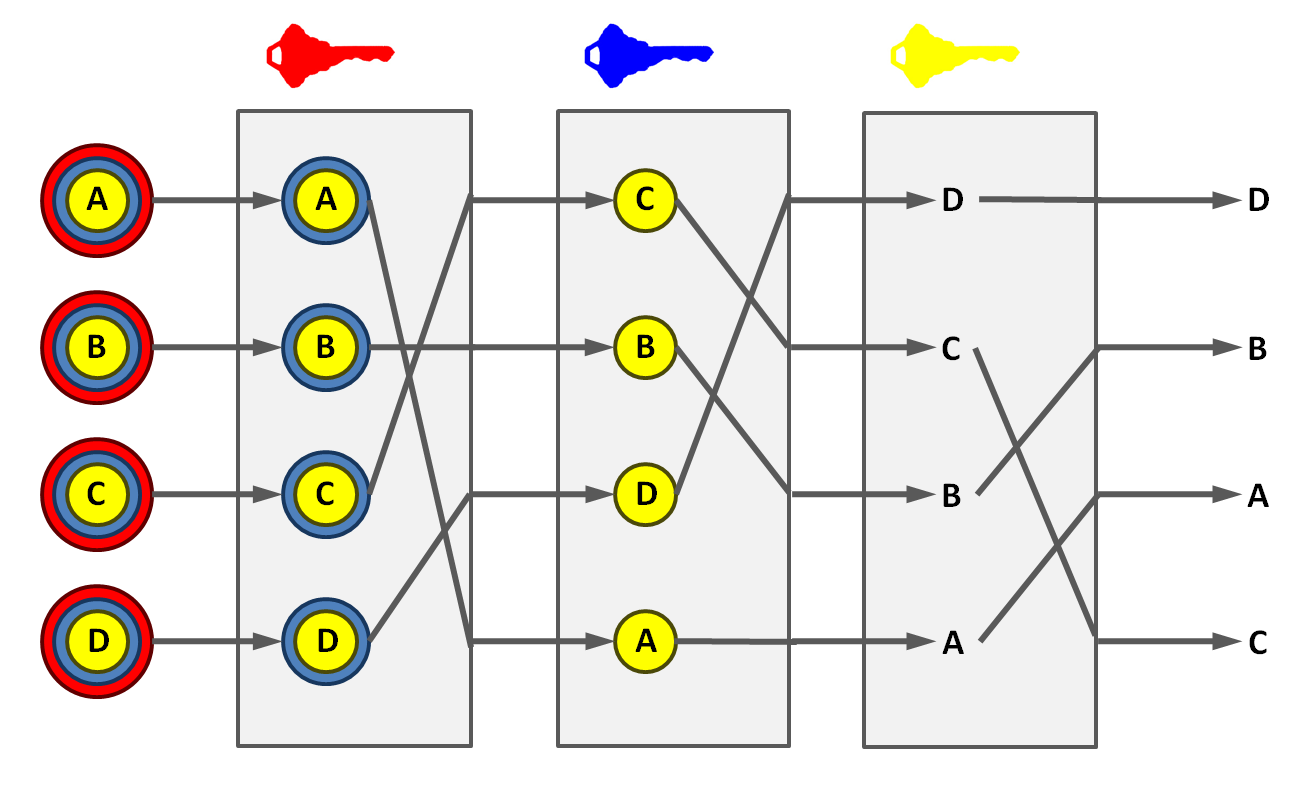
\includegraphics[width=0.7\textwidth]{imgs/Decryption_mix_net.png}
	\end{center}
	\end{minipage}
\end{frame}

\begin{frame}
	\frametitle{Old times}
	\begin{itemize}
		\item Anonymous remailers: end to end anonymity.
		\begin{itemize}
			\item Cypherpunk: remove FROM field and encrypt the mail
			\item Mixmaster: Chain of remailers.
			\item Mixminion: Mixmaster syntax with replies.
			\item nym-server: give a pseudonym to the user detached
			from his IP.
		\end{itemize}
		We'll see that this servers recalls the modern idea of
		OnionRouting.
	\end{itemize}
\end{frame}

\begin{frame}
	\frametitle{Onion Routing}
	The idea of encapsulate cyphered packets in a chain or an "onion".

	\begin{itemize}
		\item OpenNet? $\to$ Hidden services.
		\item New possibility like use a proxy to get to the normal
		internet.
	\end{itemize}
	\begin{block}{Problems}
	\begin{itemize}
		\item Performance
		\item DoS resistance.
		\item Mantain links to the users
		\item Thrustness of the routers.
		\item Confidentiality and autenticity.
	\end{itemize}
	\end{block}
\end{frame}

\begin{frame}
	\frametitle{Onion Routing (2)}

	\begin{itemize}
		\item TOR 
\includegraphics[scale=0.1]{imgs/Tor_logo}
		\begin{itemize}
			\item We'll come to this later.
		\end{itemize}
		\item i2p 
\includegraphics[scale=0.2]{imgs/I2P_logo}
		\begin{itemize}
			\item Done for eepsite(s).
			\item Not so much routers/outproxies.
		\end{itemize}
	\end{itemize}
	\begin{itemize}
		\item And what for the low latency? $\to$ \textbf{Timing attacks}.
	\end{itemize}
\end{frame}

\begin{frame}
	\frametitle{Why simulation?}
	Simulation help us in a lot of aspects:

	\begin{itemize}
		\item Compare the performances of two onion routers (p.e. i2p vs
		Tor).
		\item To compare effects of changes in the node choice
		algorithms.
		\item \textbf{Get an idea of the number of resources needed by an
		attacker and to mantain anonimity}.
	\end{itemize}
\end{frame}

\section{Tor}
\begin{frame}
	\frametitle{NSA and Tor}
	Tor was made from the naval research labs:
	\begin{itemize}
		\item Made for the anonymous control and espionage.
		\item Tor need a number of exit nodes (and routers) to lead
		anonymity to an user.
		\item if an organization use only his exit nodes it's like to
		not use them at all.
	\end{itemize}
\end{frame}

\begin{frame}
	\frametitle{The Tor revolution}
	Apparently Tor slipped from the hands of the US in the 2004.
	\begin{minipage}{.49\textwidth}

	\begin{itemize}
		\item Russia offered \$114.000 to identify and deface Tor
		anonimity.
		\item NSA now classify TOR as a menace of level
		\textit{catastrophic}.
	\end{itemize}
	\end{minipage}
	\begin{minipage}{.5\textwidth}
		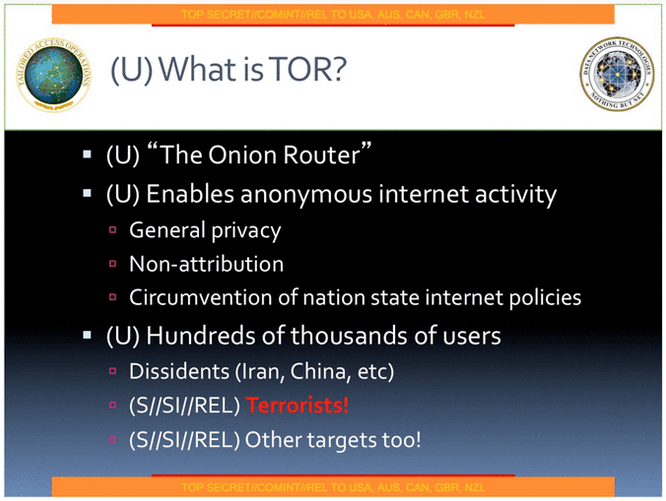
\includegraphics[scale=0.35]{imgs/nsa_tor}
	\end{minipage}
	But...nobody knows who and what is hidden under the layer of the onion.
\end{frame}
